\chapter{Evaluation}
\label{eval:svm}
\section{Hardware selection}
\label{sec:eval:hw}
The moste relevant hardware feature of processors when working on instruction scheduling is the instruction pipeline.
We are specifically interested in the fact if a instruction pipeline is a in-order or out-of-order pipeline (\Cref{sec:bg:superscalar-cpu}).
In-order processors execute the instructions in the schedule that is written in the executable file.
A out-of-order processor might reschedule the instructions in hardware.

For our experiments we have selected two different types of processors, one of each type:
\begin{itemize}
    \item 
    % \subsubsection{AArch64}
    The AArch64 hardware architecture is a 64-bit ARM architecture with a in-order superscalar pipeline.
    A \ac{cpu} that implements this hardware, and that we use for our experiment is the Arm Cortex-A53.
    We use this \ac{cpu} in the RaspberryPi 3 Model B with a Ubuntu 20.04.
    \todo{Correct Ubuntu version?}
    
    \item
    % \subsubsection{\aurora}
    The second processor is the \aurora vector processor that implements a out-of-order superscalar pipeline.
    This processor is installed via a PCI-Express slot.
\end{itemize}
    
\section{Approach Validation}
Before starting to optimize a process, it is useful to validate that there is potential for any optimizations.
Therefore, we show, that different instruction schedules can indeed have different runtimes on our target hardware.
The approach of this experiment is differs from the other experiments because it is an early experiment that took place before our pipeline was developed.
\todo{Is this sentence useful /okay?}

% select longest bb per benchmark
% longest might have the most possible schedule, so more variation in the random schedules
\Cref{sec:approach:dataset} describes the selection of benchmarks from the LLVM Test Suite.
For this experiment we select one basic block per benchmark, for which we modify its instruction schedule.
For the selection of basic blocks we use the heuristic that balances between the most executions and the longest basic blocks, which is discussed in \Cref{sec:approach:basicblock:selection}.
A high number of instructions in a basic block is typically a good indicator for a high number of possible instruction schedules for that basic block. 
A high number of executions ensures that the basic block has a high impact on the runtime of the function that it contains.

% measure the function runtime
% we measure the runtime of the function (implemented llvm passes)
% talk about impact on measurements.
We executed this experiment in a early stage and did not have a basic block extraction pipeline nor means to measure the execution time of a single basic block.
Therefore, we must execute the whole benchmark with the modified instruction schedule of a single basic block.
However, measuring the runtime of the whole benchmark, includes the execution of much overhead code, that we are not interested in.
Thus, we measure the runtime of the function that contains the basic block of interest.
This corresponds to the third method in \Cref{fig:approach:runtime_scopes}.

We implement a pass for the LLVM optimizer, to measure the runtime of a single function.
\todo{Put into approach chapter?}
The pass searches for the function that contains the selected basic block.
Then, it injects calls to the timer functions of the C++ standard library (\lstinline|std::high_resolution_clock::now|).
The calls are injected at the beginning of the given function and right before the return statement.
It injects a compilation-unit-wide global variable, and stores the measurements into this variable.
In the destructor of that compilation-unit, the pass injects code to print all the measurements.

% generate 10 different random schedules 
% do that twice
To generate different different instruction schedules, we choose the simple approach of generating random schedules.
Our random instruction scheduler works on top of a basic list scheduler.
This means, that the list scheduler selects the instructions that are ready for scheduling, and our random scheduler randomly selects one of them.
This is done until no more instructions are left.
We set the seed of the random number generator for reproducibility.

We generate instruction schedules with the seeds 0-10 for each selected basic block, \ie we generate 11 instruction schedules per basic block.
The basic block of interest might execute multiple times in the measured function for reasons discussed in \Cref{sec:approach:runtime-measurement-unit}.
We choose the shortest measured runtime per benchmark run, to ensure that we use the same execution path in our measurements.
To check that the runtime measurements are reproducible, we run the each generated instruction schedule two times.

% evaluate
We have run this experiment on the two processors described in \Cref{sec:eval:hw}.
\Cref{fig:eval:rndm:aarch64} shows a selection of experiment results.
The plots show the runtimes grouped by the different seeds for the random instruction scheduler.
Runtimes that differ between two runs more than 5\% are marked as outliers and plotted in gray.
\Crefrange*{fig:eval:rndm:aarch64:a}{fig:eval:rndm:aarch64:d} show examples where different runtimes are clearly observable for different instruction schedules.
However, this was not always observable.
\Cref{fig:eval:rndm:aarch64:e} and \Cref{fig:eval:rndm:aarch64:f} show examples where no differnce in the runtime was observable.
The average coeffecient of variation over the basic blocks is 0.035.
In summary, we see that different instruction schedules can generate measurable differences in the runtime.
This means that there is potential for improvements.
\begin{figure}
    \begin{subfigure}{0.45\textwidth}
        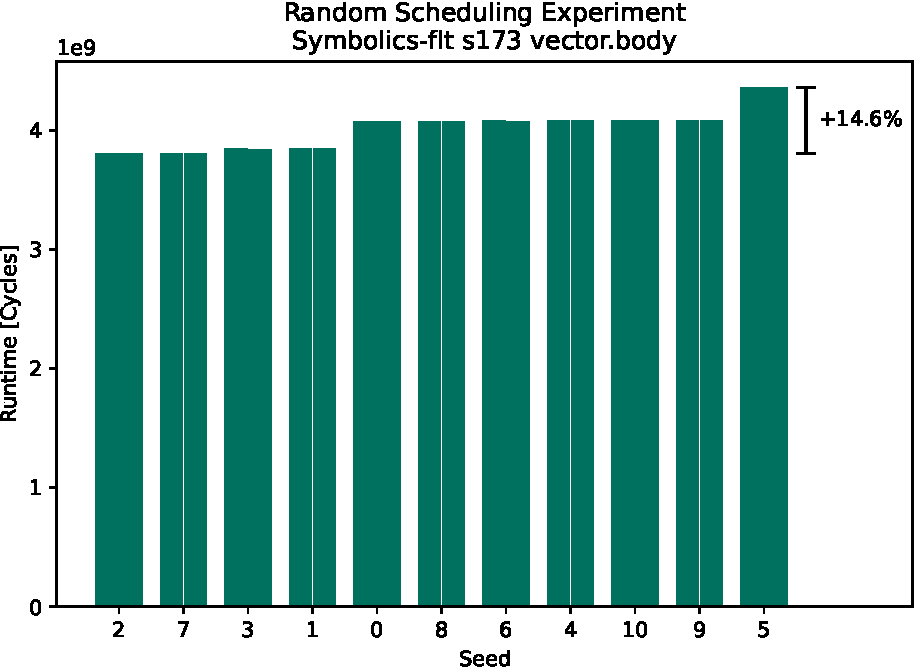
\includegraphics[width=\textwidth]{img/random-scheduling-experiment-pi-collected/Symbolics-flt-crop.pdf}
        \caption{}
        \label{fig:eval:rndm:aarch64:a}
    \end{subfigure}
    \hfill
    \begin{subfigure}{0.45\textwidth}
        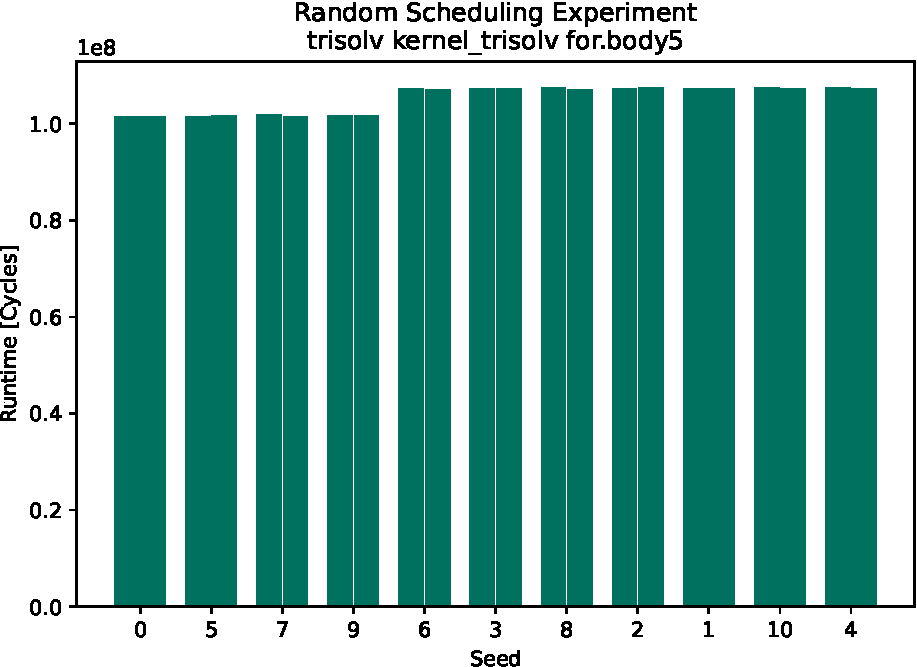
\includegraphics[width=\textwidth]{img/random-scheduling-experiment-pi-collected/trisolv-crop.pdf}
        \caption{}
        \label{fig:eval:rndm:aarch64:b}
    \end{subfigure}
    \begin{subfigure}{0.45\textwidth}
        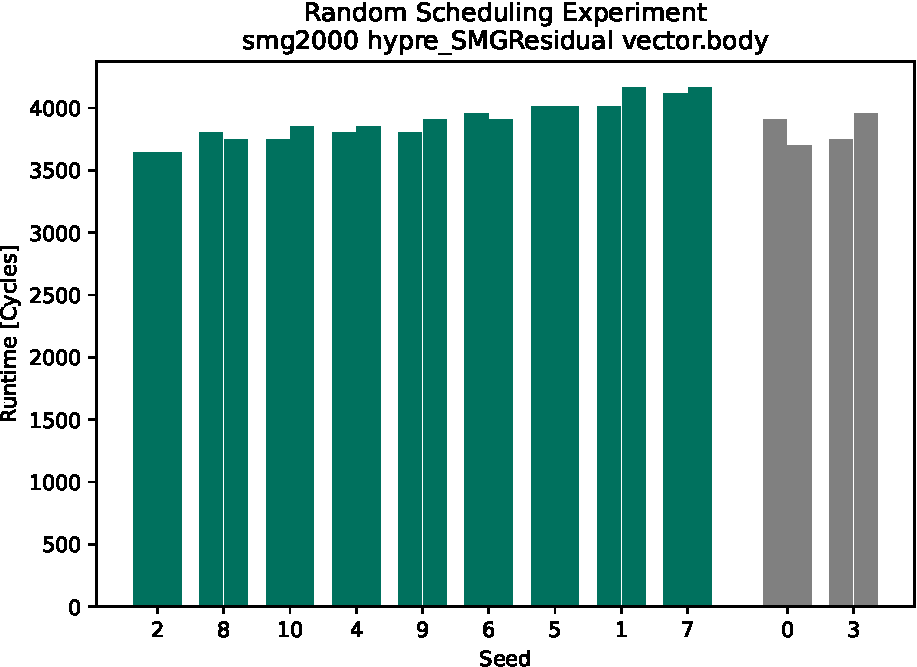
\includegraphics[width=\textwidth]{img/random-scheduling-experiment-pi-collected/smg2000-crop.pdf}
        \caption{}
        \label{fig:eval:rndm:aarch64:c}
    \end{subfigure}
    \hfill
    \begin{subfigure}{0.45\textwidth}
        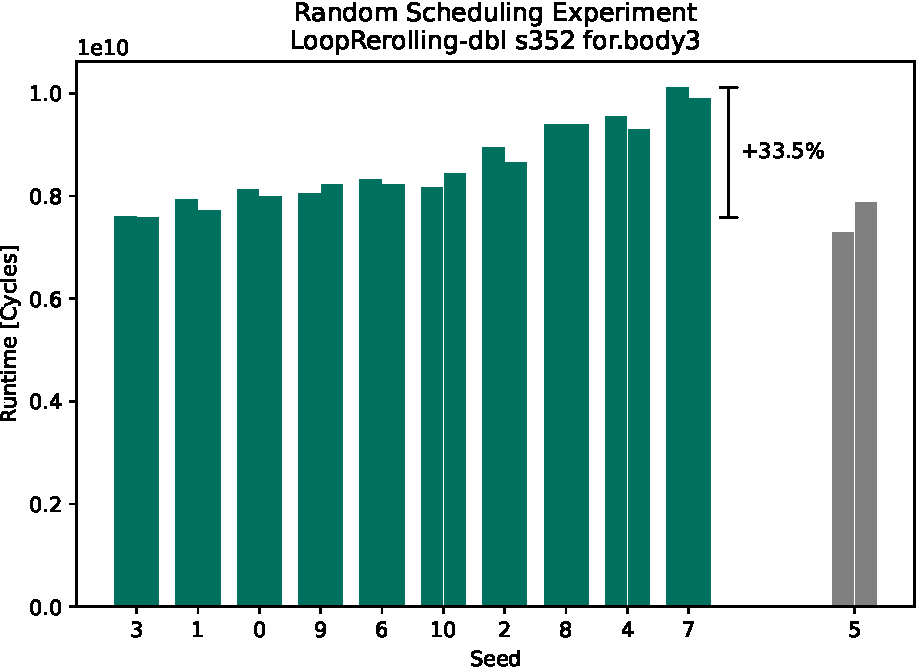
\includegraphics[width=\textwidth]{img/random-scheduling-experiment-pi-collected/LoopRerolling-dbl-crop.pdf}
        \caption{}
        \label{fig:eval:rndm:aarch64:d}
    \end{subfigure}
    \begin{subfigure}{0.45\textwidth}
        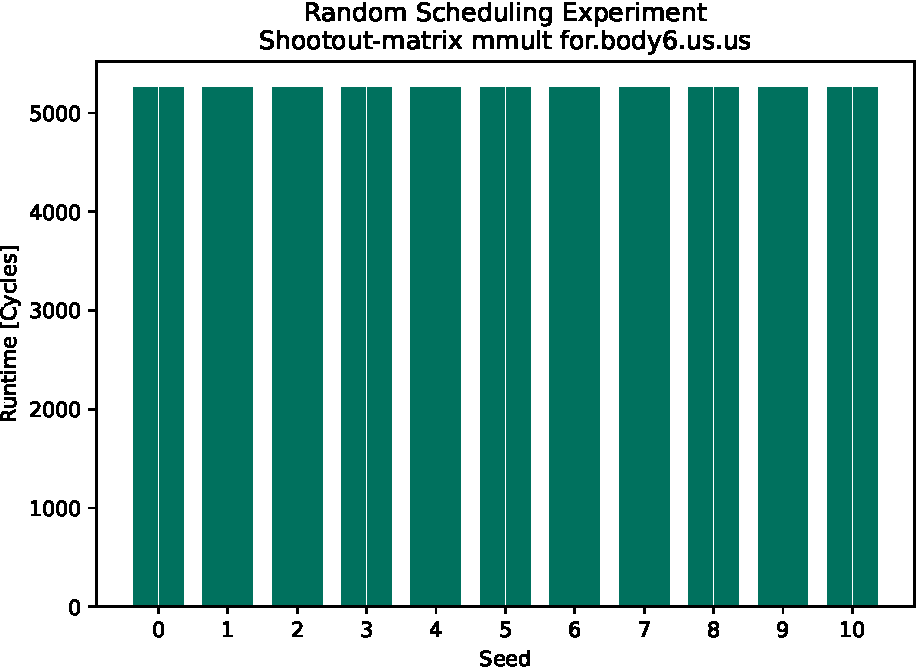
\includegraphics[width=\textwidth]{img/random-scheduling-experiment-pi-collected/Shootout-matrix-crop.pdf}
        \caption{}
        \label{fig:eval:rndm:aarch64:e}
    \end{subfigure}
    \hfill
    \begin{subfigure}{0.45\textwidth}
        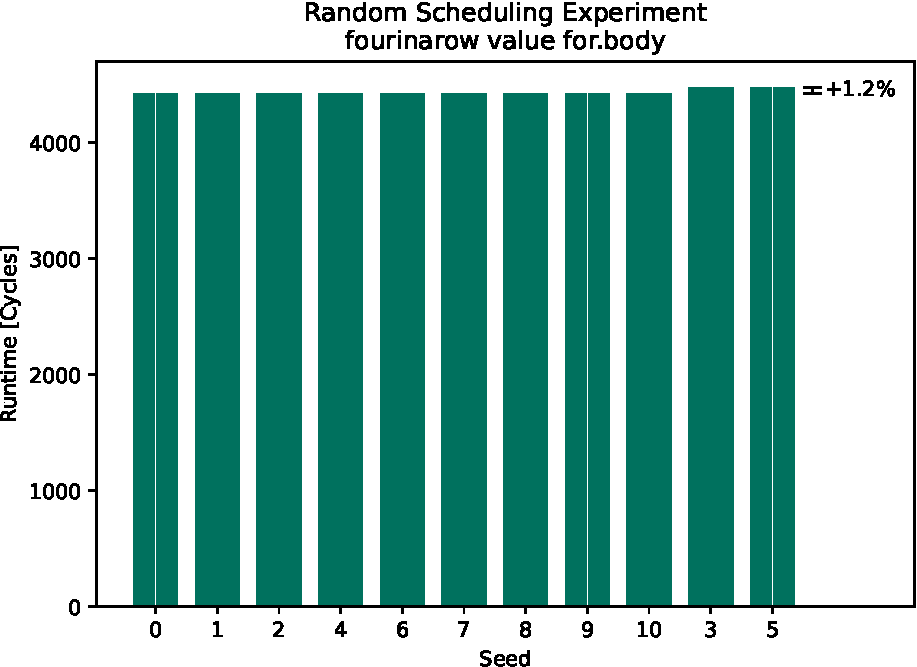
\includegraphics[width=\textwidth]{img/random-scheduling-experiment-pi-collected/fourinarow-crop.pdf}
        \caption{}
        \label{fig:eval:rndm:aarch64:f}
    \end{subfigure}
    \caption[Random Scheduling Experiment on AArch64]{Random Scheduling Experiment on AArch64:
    The bars show the runtime of a function with a random instruction schedule.
    The two runs of the instruction schedule are grouped together.
    Two runs that differ more than 5\% are marked as outliers and plotted in gray.}
    \label{fig:eval:rndm:aarch64}
\end{figure}

\Cref{fig:eval:rndm:aurora} shows a similar selection for the same experiment on the \aurora processor.
We can observe a similar outcome of the experiment.
However, as this processor cannot be interrupted by the \ac{os}, the runtimes are more stable between two runs.
No measurements in the whole example where marked as outliers.
The average coeffecient of variation over the basic blocks is 0.046.
In summary, we observe potential for optimizations on this processor.
\begin{figure}
    \begin{subfigure}{0.45\textwidth}
        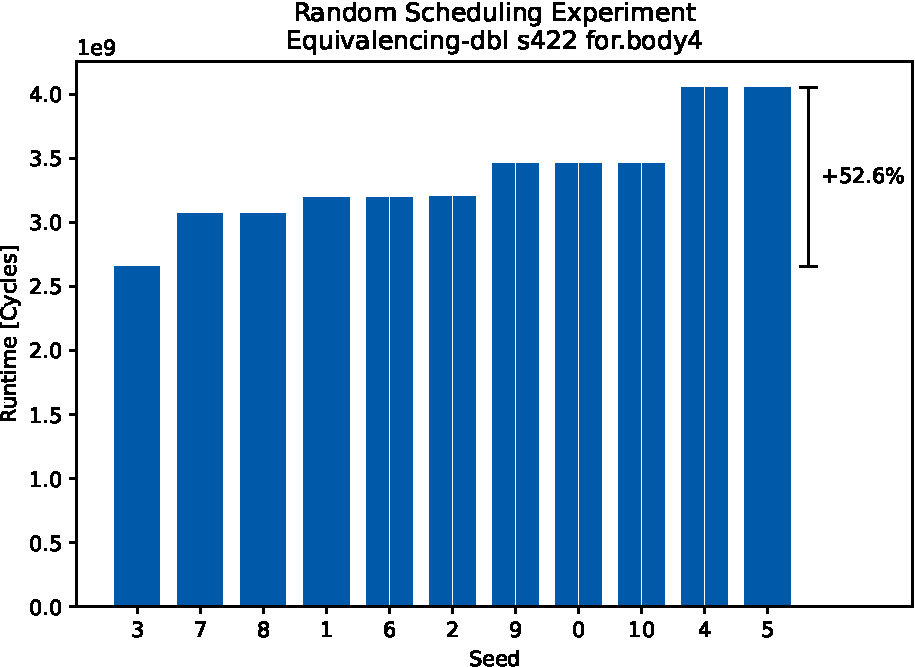
\includegraphics[width=\textwidth]{img/random-scheduling-experiment-aurora-collected/Equivalencing-dbl-crop.pdf}
        \caption{}
        \label{fig:eval:rndm:aurora:a}
    \end{subfigure}
    \hfill
    \begin{subfigure}{0.45\textwidth}
        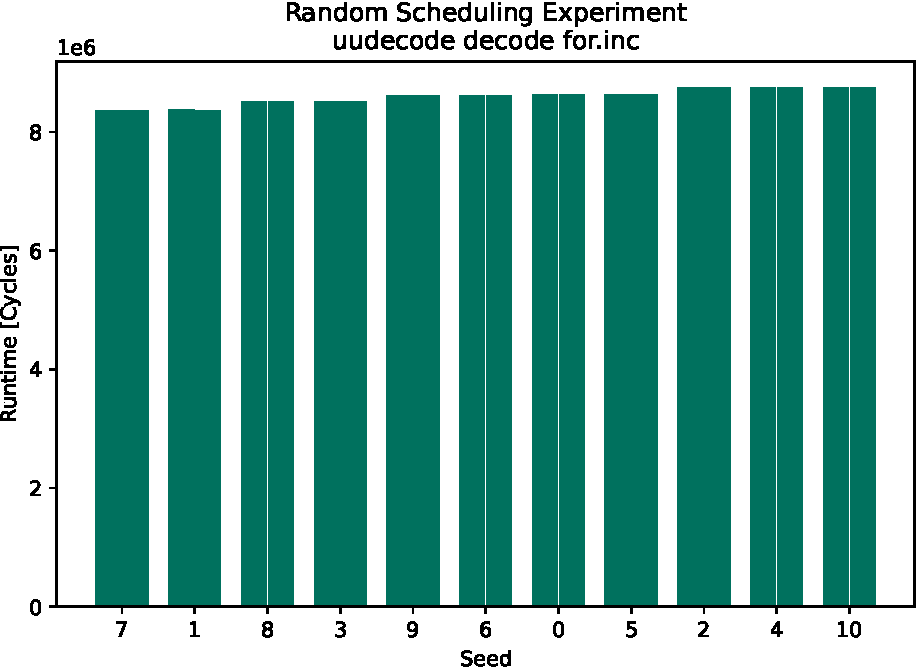
\includegraphics[width=\textwidth]{img/random-scheduling-experiment-aurora-collected/uudecode-crop.pdf}
        \caption{}
        \label{fig:eval:rndm:aurora:b}
    \end{subfigure}
    \begin{subfigure}{0.45\textwidth}
        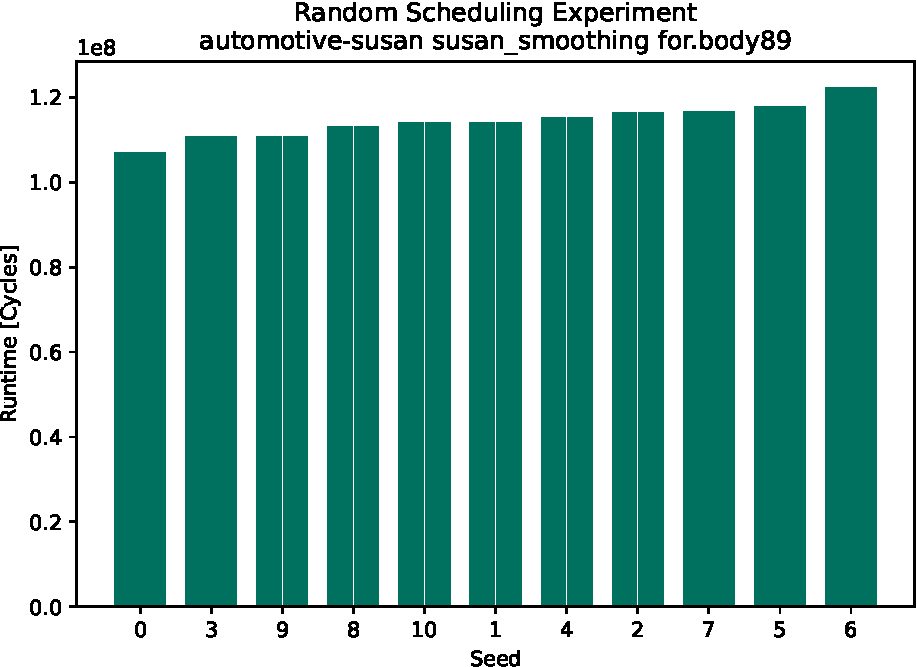
\includegraphics[width=\textwidth]{img/random-scheduling-experiment-aurora-collected/automotive-susan-crop.pdf}
        \caption{}
        \label{fig:eval:rndm:aurora:c}
    \end{subfigure}
    \hfill
    \begin{subfigure}{0.45\textwidth}
        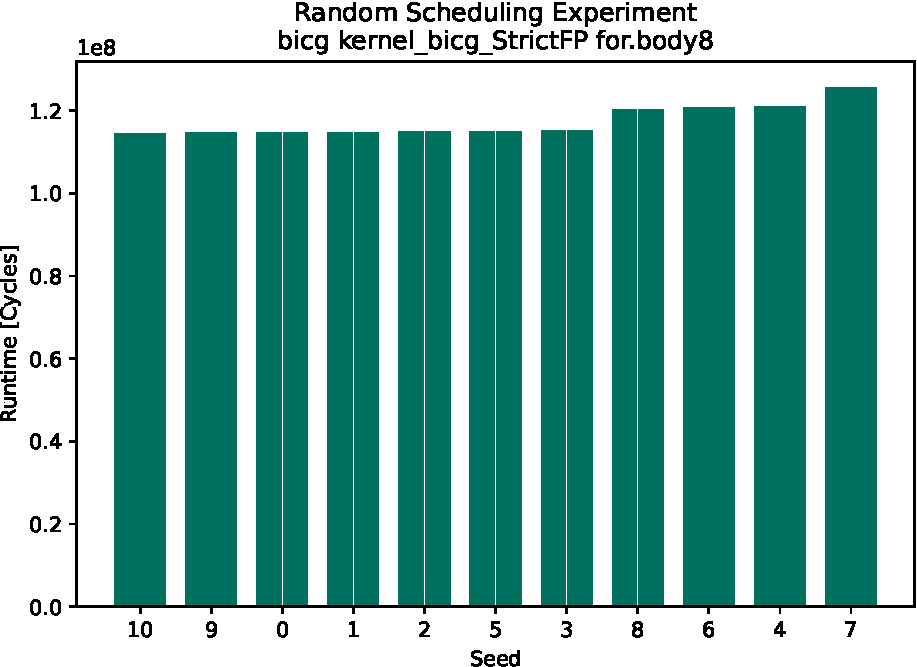
\includegraphics[width=\textwidth]{img/random-scheduling-experiment-aurora-collected/bicg-crop.pdf}
        \caption{}
        \label{fig:eval:rndm:aurora:d}
    \end{subfigure}
    \begin{subfigure}{0.45\textwidth}
        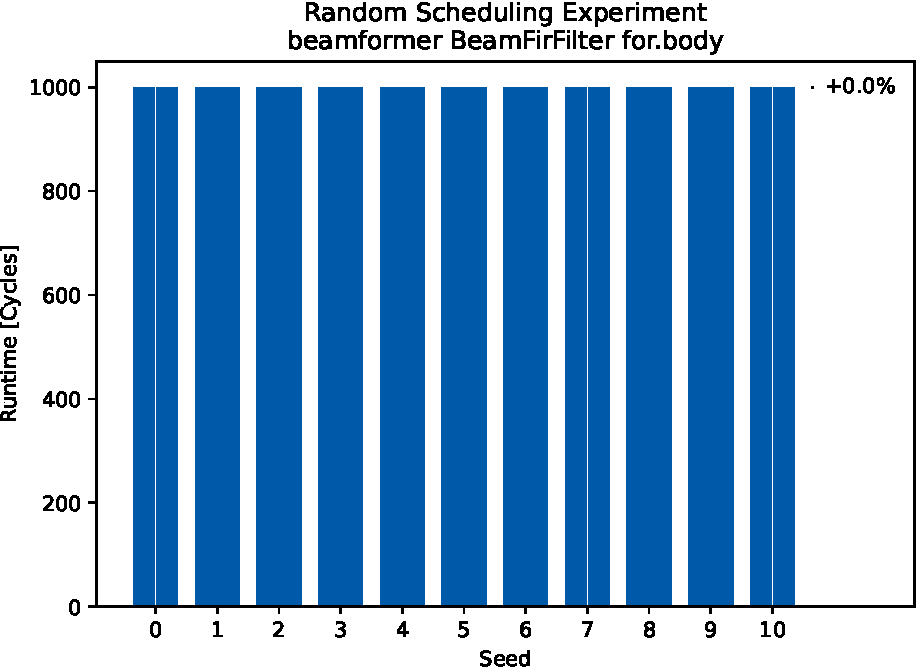
\includegraphics[width=\textwidth]{img/random-scheduling-experiment-aurora-collected/beamformer-crop.pdf}
        \caption{}
        \label{fig:eval:rndm:aurora:e}
    \end{subfigure}
    \hfill
    \begin{subfigure}{0.45\textwidth}
        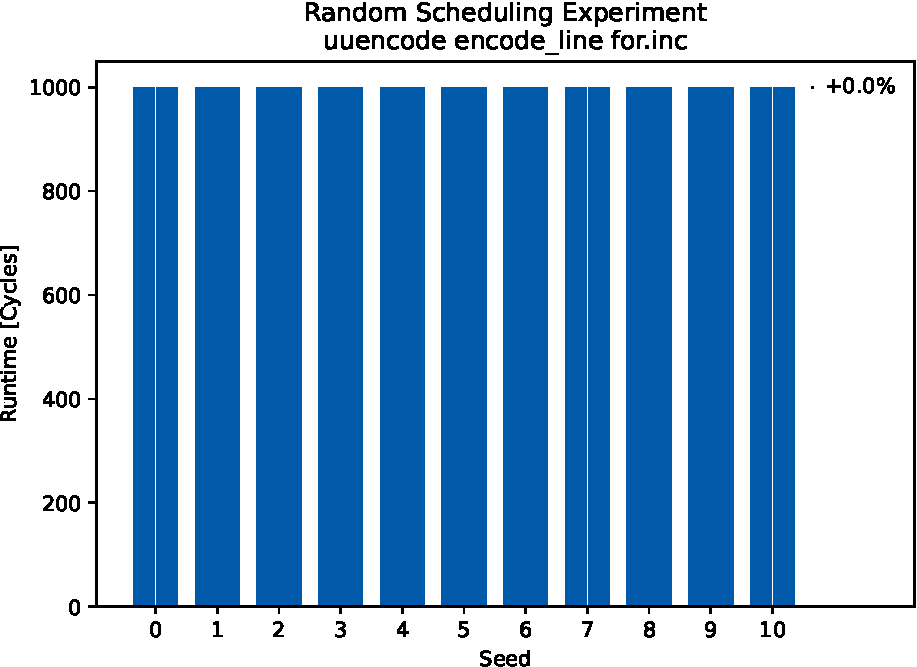
\includegraphics[width=\textwidth]{img/random-scheduling-experiment-aurora-collected/uuencode-crop.pdf}
        \caption{}
        \label{fig:eval:rndm:aurora:f}
    \end{subfigure}
    \caption[Random Scheduling Experiment on \aurora]{Random Scheduling Experiment on \aurora:
    The bars show the runtime of a function with a random instruction schedule.
    The two runs of the instruction schedule are grouped together.
    Two runs that differ more than 5\% are marked as outliers.
    However, this processor did not produce any outliers in our experiment.}
    \label{fig:eval:rndm:aurora}
\end{figure}

There are multiple possible reasons that would cause equal measurements in this experiment.
We must differntiate between reasons which mean that different instruction schedules have no effect on the runtime of the basic block and reasons that have its origin in the experiment setup.
We cannot do anything about the former.
Actually, the motivation for this experiment was to verify, that the former reasons do not dominate all the instruction schedules.
There are multiple possibilities for the latter reasons, that have ther origin in the experiment setup:
\begin{itemize}
    \item The basic block for which we manipulate the instruction schedule might have a low influence on the runtime of the function.
        We tried to minimize this effect by choosing basic blocks that are often executed.
    \item Our random instruction scheduler works on top of LLVM.
        LLVM makes, in this stage of the back-end, still use of pseudo instruction that are not represented in the binary.
        This means that schedules that we see as different schedules, might actually not differ in the binary.
    \item There are short functions with a short execution time.
        We observed few changes in the runtime when the measured execution time is below 10,000 processor cycles.
        The underlying timer of the C++ standard library might not be able to measure such short time periods.  
\end{itemize}
However, the experiment is still valid, because we show that we are able to influence the runtime by manipulating the instruction schedules.

In summary, we observe different runtimes for different instruction schedules and the results are reproducible over multiple runs.
This is not true for all basic blocks, but the goal of this experiment was to show the existence of an effect of the instruction schedule on the runtime.
These results motivate the further research on optimizing instruction schedules for these two processors.

\section{MCTS Schedule Search}
Shows that there is $~8\%$ range for improvements that we have found.

\section{Machine Learning Schedule Generation}
\subsection{Look-Up Model}
\subsection{Support Vector Regression}
\subsection{Neural Network}

Compare speedup with complexity of the problem (number of possible schedulings) vs speedup

Compare CPU Architectures, In-Order vs Out-Of-Order (\url{https://en.wikipedia.org/wiki/Out-of-order_execution})
Here, check speedup vs basic block length, to see if ooo processors perform worse on long basic blocks where it can't see too many instructions ahead

Might be interesting for the discussion: \url{http://www.irisa.fr/alf/downloads/PMA/p241-mcfarlin.pdf}

Mean vs. Median discussion in runtime measurements

\begin{itemize}
    \item Hardware
    \begin{itemize}
        \item Arm Cortex-A53
        \item NEC Aurora
    \end{itemize}
\end{itemize}



Run \ac{mcts} more iterations, because the rest of the schedules still contain many random decision and we can see, that a single decision can make a big difference.
